\begin{statement}{4}
  Compute the barycentric weights numerically using $n + 1$ equally spaced nodes in $[-1, 1]$
  for $n = 30, 60, 90$. On a single graph, plot their absolute values as a function of $t_i$
  (which always ranges between $-1$ and $1$) using a log-linear scale.
\end{statement}

\begin{solution}
  Modifying the barycentric interpolation function to return only the vector of weights
  \lstinputlisting{scripts/algorithms/barycentric-weights.m}
  we plot the absolute values of the weights using a log-linear scale.
  \lstinputlisting{scripts/problems/problem-04.m}
  \begin{figure}[H]
    \centering
    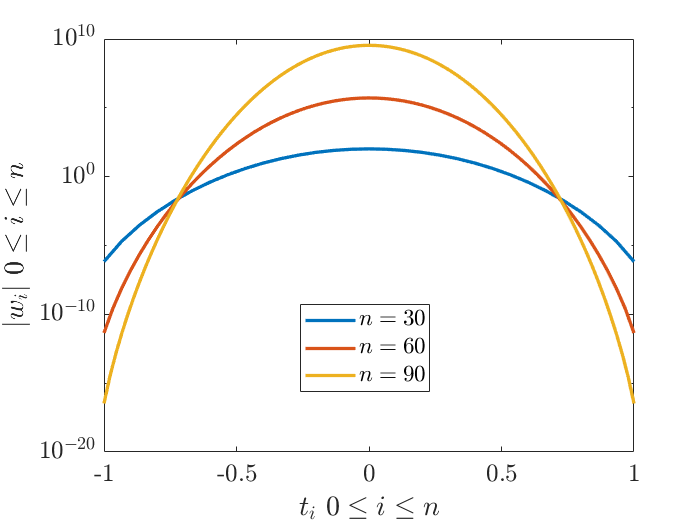
\includegraphics[scale=0.5]{graphics/plot-04.png}
    \caption{Absolute value of barycentric weights}
  \end{figure}
\end{solution}